%%%%%%%%%%%%%%%%%%%%%%%%%%EJERCICIO 5 %%%%%%%%%%%%%%%%%%%%%%%%%%%
	
	\textbf{Ejemplo 5}\\
	Hallar la distribución del pago número 125 periodo mes vencido (valor de los intereses y del capital amortizado), en una amortización de  2'000.000 COP, mediante pagos mensuales durante 20 años, suponiendo una tasa del 30\% nominal anual mes vencido.
	
	%\newpage %USAR SOLO SI EL SOLUCIÓN QUEDA SOLO Y ES NECESARIO BAJARLO A LA SIGUIENTE PAGINA
	
	\textbf{Solución 5.}\\
	%La tabla ira centrada
	\begin{center}
		\renewcommand{\arraystretch}{1.5}% Margenes de las celdas
		%Creación de la cuadricula de 3 columnas
		\begin{longtable}[H]{|p{0.5\linewidth}|p{0.5\linewidth}|}
			%Creamos una linea horizontal
			\hline
			%Definimos el color de la primera fila
			\rowcolor[HTML]{FFB183}
			%%%%% INICIO ASIGNACIÓN PERIODO FOCAL %%%%%%%
			%%%%%%%%%% INICIO TITULO
			%Lo que se hace aquí es mezclar las 3 columnas en una sola
			\multicolumn{2}{|c|}{\cellcolor[HTML]{FFB183}\textbf{1. Asignación período focal}}   \\ \hline
			%%%%%%%%%% FIN TITULO
			%%%%% INICIO DECLARACIÓN DE VARIABLES %%%%%%%
			\multicolumn{2}{|c|}{$pf = 0 \textit{ ptv}$}\\ \hline
			%%%%%%%%%% INICIO TITULO
			%Lo que se hace aquí es mezclar las 3 columnas en una sola
			\multicolumn{2}{|c|}{\cellcolor[HTML]{FFB183}\textbf{2. Declaración de variables}}   \\ \hline
			%%%%%%%%%% FIN TITULO
			%%%%%%%%%% INICIO DE MATEMÁTICAS
			%Cada & hace referencia al paso de la siguiente columna
			$VP =  2$.$000$.$000 \hspace{1mm} COP$  				& $R = ? \hspace{1mm} COP    $  \\
			$j  \equiv  30\%  \hspace{1mm} namv$      	& $I = ? \hspace{1mm} COP    $ \\
			$i \equiv  2,5\% \hspace{1mm} pmv$           & $A = ? \hspace{1mm} COP     $ \\ 
			$n = 125 \hspace{1mm} pmv$          & $ $ \\ \hline
			%%%%%%%%%% FIN DE MATEMÁTICAS
			%%%%% FIN DECLARACIÓN DE VARIABLES
			
			\rowcolor[HTML]{FFB183}
			\multicolumn{2}{|c|}{\cellcolor[HTML]{FFB183}\textbf{3. Diagrama de flujo de caja}} \\ \hline
			\multicolumn{2}{|c|}{ 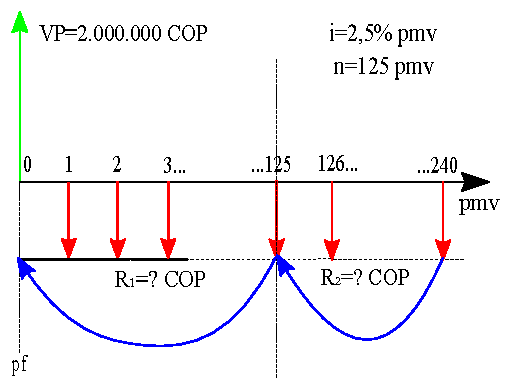
\includegraphics[trim=-78 -5 -78 -5]{7_Capitulo/img/ejemplos/5/5_1.pdf} }   \\ \hline
			%%%%% INICIO FLUJO DE CAJA
			\rowcolor[HTML]{FFB183}
			\multicolumn{2}{|c|}{\cellcolor[HTML]{FFB183}\textbf{4. Declaración de fórmulas}} \\ \hline
			%%%%%%%%%%%%% FIN INSERCIÓN DE IMAGEN
			%%%%%FIN FLUJO DE CAJA
			
			\multicolumn{2}{|c|}{ $VP = R \frac{1-(1+i)^{-n}}{i} $ Valor presente serie uniforme vencido }   \\ 
			\multicolumn{2}{|c|}{ $I = P \hspace{1mm} i $ Interés periódico }   \\ 
			\multicolumn{2}{|c|}{ $A = R - I $ Amortización a capital, una vez descontados los intereses de la cuota R }   \\ \hline
			
			%%%%%% INICIO DESARROLLO MATEMÁTICO
			\rowcolor[HTML]{FFB183}
			%%%%%%%%%%INICIO TITULO
			\multicolumn{2}{|c|}{\cellcolor[HTML]{FFB183}\textbf{5. Desarrollo matemático}}       \\ \hline
			%%%%%%%%%% FIN TITULO
			%%%%%%%%%% INICIO MATEMÁTICAS
			\multicolumn{2}{|C{\linewidth}|}{
				Como todos los pagos son iguales, entonces el valor del pago 125 se obtiene de la siguiente ecuación:
				
			
				$  2$.$000$.$000 \hspace{1mm} COP  = R \frac{1-(1+ 0,025)^{-240}}{0,025} $ Ecuación de valor
			
				  $Donde \hspace{1mm} R =  5$.$133,78 \hspace{1mm} COP$
			
				Por otra parte se sabe que la porción de la cuota 125 pmv que se utiliza para pagar intereses es igual a la tasa, multiplicada por la deuda que queda inmediatamente después de haberse efectuado el pago número 124 pmv. Entonces, para hallar la deuda, en ese momento, debemos calcular el valor presente de los pagos que faltan por hacer.
				
				Como en total hay 240 pagos y se han hecho 124 entonces faltan por hacer 116 pagos. El valor presente de estos pagos en el punto 124 será:
				
				$ VP =   5$.$133,78 \hspace{1mm} COP  \frac{1-(1+ 0,025)^{-116}}{0,025} =   1$.$891$.$004,92 \hspace{1mm}  COP\hspace{1mm} deuda \hspace{1mm}en\hspace{1mm} la \hspace{1mm}cuota \hspace{1mm}124 $ 
				
				Y los intereses serán:
				
				$ I= (  1$.$891$.$004,92 \hspace{1mm} COP)(0,025) =  47$.$275,12 \hspace{1mm} COP$
				
				Finalmente, la amortización será igual a la cuota menos intereses
				
				$ A= (  5$.$133,78 \hspace{1mm} COP)-( 47$.$275,12 \hspace{1mm} COP) =   2$.$858,66 \hspace{1mm} COP$
				
			}\\ \hline
			
			%%%%%%%%%% FIN MATEMÁTICAS
			%%%%%% FIN DESARROLLO MATEMÁTICO
			%%%%%% INICIO RESPUESTA
			\rowcolor[HTML]{FFB183}
			%%%%%%%%%%INICIO TITULO
			\multicolumn{2}{|c|}{\cellcolor[HTML]{FFB183}\textbf{6. Respuesta}}   \\ \hline
			%%%%%%%%%% FIN TITULO
			%%%%%%%%%% INICIO RESPUESTA MATEMÁTICA
			\multicolumn{2}{|c|}{ 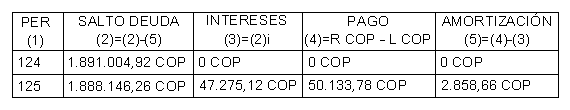
\includegraphics[trim=-78 -5 -78 -5]{7_Capitulo/img/ejemplos/5/5_2.pdf} }   \\ \hline
			%\multicolumn{2}{|C{\textwidth}|}{
			%	$P_R =  COP \hspace{1mm} 4.860.245$
			%}  \\ \hline
			
			
			%%%%%%%%%% FIN MATEMÁTICAS
			%%%%%% FIN RESPUESTA
		\end{longtable}
		%Se crean dos lineas en blanco para que no quede el siguiente texto tan pegado
		%\newline \newline %USARLO SI CREES QUE ES NECESARIO
	\end{center}
	%%%%%%%%%%%%%%%%%%%%%%%%%%FIN EJERCICIO 5 %%%%%%%%%%%%%%%%%%%%%%%%%%%